\section{Deep learning and Protein Contact Prediction}

    \subsection{Fully-convolutional networks}

        As a reminder, a fully-convolutional network is a neural network capable
        of handling variable sized input. Therefore, the dynamic input dimensions
        cannot be processed by a fully-connected neural layer.
        An example of such an architecture is DeepCov~\cite{doi:10.1093/bioinformatics/bty341},
        a deep neural network composed only of 2D convolutional layers and an additional
        maxout input layer. A maxout layer is made of a convolutional layer, followed
        by a max-pooling operation. Dimensions of intermediate feature maps are preserved
        by convolutions using a stride of one and a "same-padding". In most deep learning
        libraries, padding of type "same" refers to the padding applied by convolutional layers
        to maintain the sizes of spatial (convoluted) dimensions.
        In DeepCov, the only features are the covariance matrices as computed
        in equation \ref{covariance}.

        The approach described in the DNCON2 paper~\cite{doi:10.1093/bioinformatics/bty341}
        also implements convolutional layers with dynamic spatial dimensions.
        Additionaly to that, the fuzziness of residue contact definition is handled
        by training one fully-convolutional neural network per contact threshold.
        More specifically, five networks are trained to ouput contact maps at 6, 7.5, 8, 8.5 and 10 \AA{}
        thresholds, respectively. These five are stacked on top of a sixth network in charge
        of refining and combining the preditions into a final contact map at a threshold of 8 \AA{}.

    \subsection{Residual Networks (ResNets)}

        As described in section \ref{backpropagation} about backpropagation,
        the loss gradient with respect to the parameters of a specific layer
        is computed as the product of many other mathematical entities
        (vectors, scalars, matrices, etc.), and the number of factors in such
        a product grows linearly with the number of operations applied after
        current layer. When this number is too large, some layers may be
        updated with numerically unstable gradients.

        A widely used solution is to add
        residual connections~\cite{DBLP:journals/corr/HeZRS15}~\cite{residual network}
        to the architecture. The latter can thus no longer be viewed as
        a regular composition of functions and must take into account
        the residual mapping at the end of each residual block.
        The output $Y^{(r)}$ of residual block $k$ should now
        be formalized with a more general form:

        \begin{equation}
            Y^{(r)} = f\big(X^{(r)}, \{W^{(p)}\}_p\big)
        \end{equation}

        where $W^{(p)}$ are the weights of a layer $p$ in block $k$.
        Residual mappings can be implemented in several ways and figure \ref{resnet}
        illustrates one of them.

        \begin{figure}[H]
            \begin{center}
                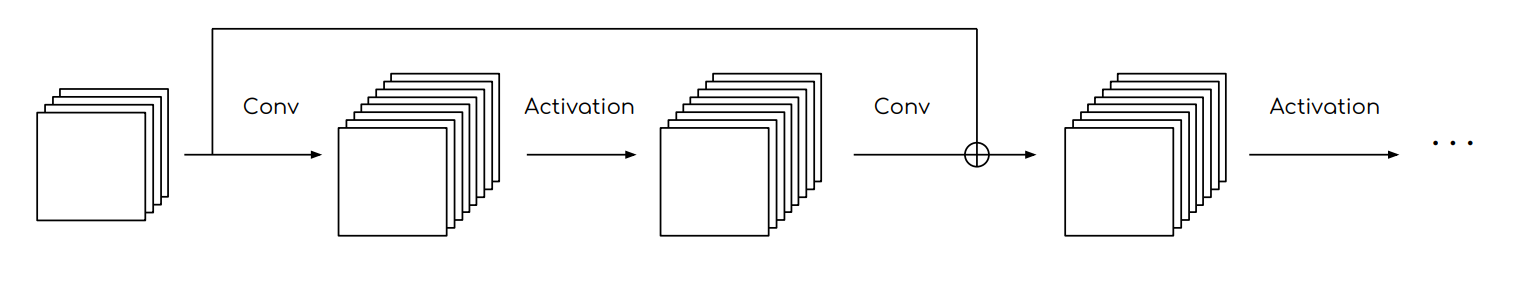
\includegraphics[width=\textwidth, keepaspectratio]{imgs/resnet.png}
                \caption{Illustration of a residual connection in a convolution
                neural network. For the element-wise sum to work, the input and output
                of the residual block are required to be of the same shape.}
                \label{resnet}
            \end{center}
        \end{figure}

    \subsection{Deep fully-convolutional residual networks}

        Most successful methods rely on very deep architectures with residual mappings.
        One-dimensional features are processed by one-dimensional residual network
        before being concatenated with two-dimensional features. The resulting tensor
        is the input of a two-dimensional residual network.
        Examples of such approach is DeepContact~\cite{DeepContact} and the state-of-the-art
        RaptorX-contact predictor~\cite{DeepContact}. Both methods rely on CCMPred contact
        prediction, solvent accessibility and secondary structure prediction.
        Additionally to CCMPred, DeepContact incorporates EVFold predictions together
        with the rest of the two-dimensional features. Also, global features (e.g. the number
        of effective sequences) are tiled and concatenated with other features: this does
        not impact the fully-convolutional property of DeepContact because global features
        are invariant to the protein length. 
        The largest difference in the two methods lies in the depth of the networks:
        9 convolutional layers for DeepContact and 60-70 layers for RaptorX-contact.
        It most be noted that RaptorX-contact architecture is not fully-convolutional
        since zero-padding is applied to feature maps when more than one protein
        is processed in a batch.

    \subsection{U-net architecture}

        In PconsC4~\cite{Michel383133}, the model is partly built on top of the U-net
        architecture~\cite{DBLP:journals/corr/RonnebergerFB15}, and trained on a set
        of 2891 proteins retrieved from PDB. Features are divided in one-dimensional
        inputs including one-hot-encoded amino acids, self-information and
        partial entropies, and two-dimensional inputs including mutual information,
        normalized mutual information and cross-entropy.
        For both mutual information and normalized mutual information,
        average product correction is applied.
        One-dimensional features are convoluted through one-dimensional residual networks~\index{residual network},
        concatenated and finally reshaped to two-dimensional maps with an outer product.
        After reshaping, the intermediary feature maps are concatenated with the
        two-dimensional features and the whole is used as input to the U-net architecture.

        Models designed for semantic segmentation problems (including PCP) have been shown
        to gain significant performance when additional connections are allowed between
        layers close to the network's input and layers close to the network's output~\cite{huang2017densely}.
        U-net architectures develop this idea: they have a somehow symmetric structure made of two sub-networks
        that compress and decompress the information, respectively.
        The first sub-network successively alternates between convolutional transformations
        and max-pooling, while the second sub-network alternates between convolutional
        transformations and upsampling. Similarly to autoencoders, the features maps
        processed the middle layers or of much smaller dimensionality than input or output tensors.
        To prevent the whole architecture from forgetting contextual information due to
        compression, shortcut connections are added between tensors of identical dimensionality.
        Contrary to residual networks, these shortcut connections are implemented by
        concatenation instead of addition. Due to the max-pooling and upsampling operations,
        the width and height of input images should preferrably be a power of two.
        Because PconsC4 model outputs entire contact maps, and because proteins are
        of variable length by nature, input feature maps of a particular protein are zero-padded
        to the smallest power of two that is larger than the protein length.

    \subsection{Dense networks (DenseNets)}

        DenseNet: \cite{huang2017densely}

        \begin{figure}[H]
            \begin{center}
                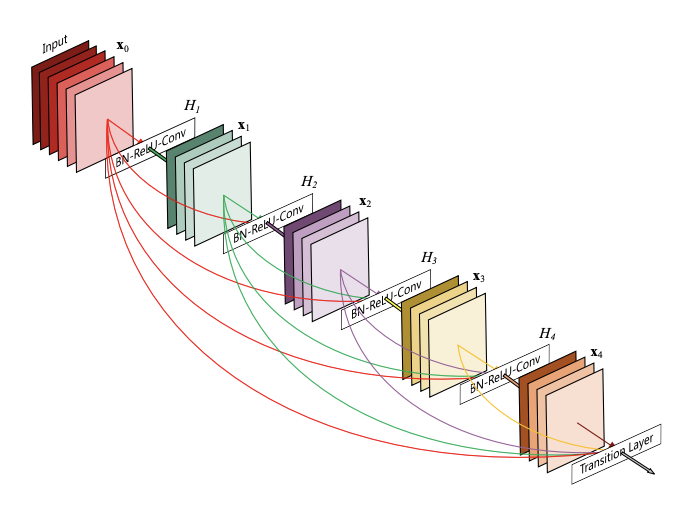
\includegraphics[width=\textwidth, keepaspectratio]{imgs/densenet.png}
                \caption{Illustration of a dense block inside a DenseNet.
                All layer entry points and outputs belonging to a dense block are connected
                by residual mappings.}
                \label{densenet}
            \end{center}
        \end{figure}



    \todo{TiramiProt: \cite{TsardakasRenhuldt1228846}}

    \todo{DeepConPred2: \cite{DeepConPred2}}

    \todo{plmConv: \cite{golkov2016protein}}

    Benchmark with both accuracy and standard deviation w.r.t. proteins.


    \todo{Deep architectures in PCP: \cite{di2012deep}}

    \begin{table}[H]
        \centering
        \resizebox{\textwidth}{!}{
        \begin{tabular}{lccc}
            \hline
             & Training set size & Fully-convolutional & \# non-linearities \\
            \hline
            \hline
            DNCON2 & 1230 & - & 6 \\
            DeepCov & 6003 & $\top$ & 14 \\
            plmConv & - & - & -\\
            DeepConPred2 & - & - & - \\
            DeepContact & - & $\top$ & 9 \\
            PconsC4 & 2891 & $\bot$ & \\
            TiramiProt & 2891 & $\bot$ & 16 \\
            RaptorX-Contact & - & $\bot$ & 60-70 \\
            \hline
        \end{tabular}
        }
        \captionof{table}{Overview of different deep learning models for PCP.}
        \label{overview}
    \end{table}